%!TEX root = ../main.tex

\chapter{HARQ}
\label{chp:analysis}

\section{Concurrent processes limit}

One of the problems highlighted by the \ac{3GPP} technical report \cite{3gpp-tr-38.811} on the matter of non-terrestrial networks regards the maximum number of concurrent \ac{HARQ} processes. 

\subsection{Processes explained}
The details of \ac{HARQ} protocol implementation in the 5G \ac{NR} standard is extensively treated in many publications such as \cite{harq-wireless-communications-survey}. However, for the purpose of understanding what is a harq process and how it affects the throughput in a non-terrestrial scenario, a brief overview of a few key concepts is enough.

\begin{figure}[ht]
    \centering
    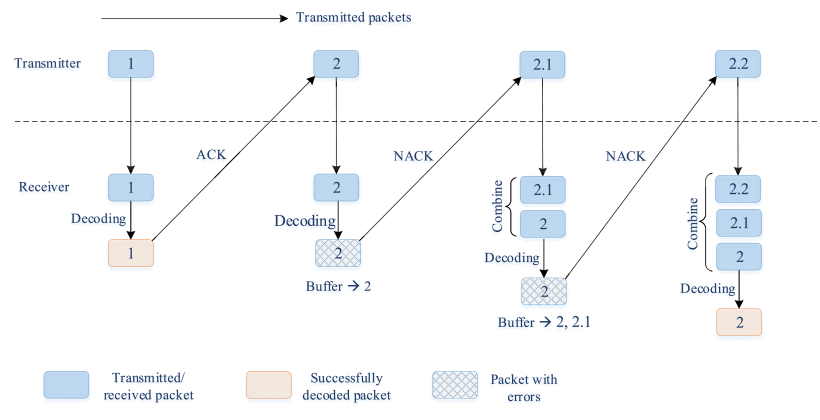
\includegraphics[width=0.7\textwidth]{res/harq-retx-scheme.png}
    \caption{\ac{HARQ} retransmission diagram \cite{harq-wireless-communications-survey}}
    \label{fig:harq_retx_scheme}
\end{figure}


\paragraph{}\ac{HARQ} is a stop-and-wait protocol, meaning that it is designed to wait for the arrival of previous packet's \ac{ACK} before sending the new one. While this enforces the delivery of ordered packets, it also brings the downside of severely underutilizing the channel capacity, wasting resources that could potentially be used for transmission instead \cite{3gpp-ts-38.214}.

This limitation can be overcome by the introduction of multiple concurrent processes.

A \ac{HARQ} process starts when a \ac{TB} is passed to the \ac{HARQ} entity and finishes when the \ac{ACK} relative to that same \ac{TB} is received by the sender. After the \ac{ACK} is correctly received, the next \ac{TB} starts being processed. Considering a link with propagation delay $\tau_p$, the minimum active time for a process is therefore $2\tau_p$. 

5G \ac{NR} standard allows the base station to configure the maximum number of concurrent \ac{HARQ} processes each user can have, with the default value being 8 and the maximum 16 \cite{3gpp-ts-38.300}. 

\paragraph{Example} Consider an example scenario where each process tries to send a \ac{TB} at the maximum possible rate, every $2\tau_p$, to a \ac{LEO} satellite orbiting at 2.000Km, therefore having $\tau_p\approx6$ms. Assuming the best possible conditions with no need for retransmissions and assuming that the base station grants the \ac{UE} to the best possible clearance of 16 concurrent processes, the total send rate is of 16 transfer blocks every 12ms. In order to target a throughput of 50Mbps, the block size must therefore be of at least $$\frac{\textit{target throughput} \times 2\tau_p}{\textit{number of processes}} = 37,5Kb$$

This is not a realistic option even for terrestrial networks, where the \ac{SNR} poses a less stringent constraint, let alone for non-terrestrial ones.


\todo{Problem of harq concurrent processes: each process has a timeout of 100ms and the max number of processes is 100. A higher number of concurrent processes crashes the simulator. As the propagation delay increases and the sending interval decreases, we are forced to keep more harq processes concurrently active, therefore reducing the number of leftover slots for additional processes. Once we reach the critical value of 100, any other packet will crash the simulator.
So, as we increase the throughput, we must also increase the number of harq processes, since there are mote packets concurrently in flight.}

\todo{investigate the latency problem at 13ms propagation delay}
\todo{explain how harq works}